\documentclass{article}
\usepackage[preprint]{neurips_2025}
\usepackage[utf8]{inputenc}
\usepackage[T1]{fontenc}
\usepackage{hyperref}
\usepackage{url}
\usepackage{booktabs}
\usepackage{amsmath,amsfonts,amssymb}
\usepackage{graphicx}
\usepackage{microtype}
\usepackage{xcolor}
\usepackage{multirow}
\usepackage{array}
\usepackage{caption}
\usepackage{subcaption}
\usepackage{wrapfig}
\usepackage{enumitem}
\usepackage{pifont}
\setlist{itemsep=1pt,topsep=2pt}
\captionsetup{font=small,labelfont=bf}
\hypersetup{colorlinks=true,linkcolor=blue!50!black,citecolor=blue!50!black,urlcolor=blue!50!black}
\graphicspath{{figures/}}
\newcommand{\miouOurs}{65.85}
\newcommand{\ciOurs}{[64.1, 67.3]}
\newcommand{\miouOfficial}{66.01}
\newcommand{\ciOfficial}{[64.3, 67.5]}
\newcommand{\miouVic}{65.02}
\newcommand{\ciVic}{[63.4, 66.8]}
\newcommand{\miouMis}{66.29}
\newcommand{\ciMis}{[64.5, 67.9]}
\newcommand{\miouCoco}{39.99}
\newcommand{\ciCoco}{[38.8, 41.0]}
\newcommand{\miouOursOracle}{72.16}
\newcommand{\ciOursOracle}{[70.6, 73.6]}
\newcommand{\miouCocoOracle}{50.41}
\newcommand{\ciCocoOracle}{[49.0, 51.3]}
\newcommand{\miouOursCoarse}{18.72}
\newcommand{\ciOursCoarse}{[18.2, 19.5]}
\newcommand{\dOfficial}{+0.16}
\newcommand{\dciOfficial}{[-0.25, +0.58]}
\newcommand{\dVic}{-0.82}
\newcommand{\dciVic}{[-2.32, +0.56]}
\newcommand{\dMis}{+0.44}
\newcommand{\dciMis}{[-1.19, +2.05]}
\newcommand{\dOracle}{+6.32}
\newcommand{\dciOracle}{[+5.32, +7.47]}
\newcommand{\dCombo}{-0.15}
\newcommand{\dciCombo}{[-0.83, +0.60]}
\newcommand{\dCocoOracle}{+10.42}
\newcommand{\dciCocoOracle}{[+9.46, +11.19]}
\newcommand{\dVicMis}{+1.26}
\newcommand{\dciVicMis}{[-0.35, +2.94]}
\newcommand{\eCorrectOurs}{67.1}
\newcommand{\eBgOurs}{30.0}
\newcommand{\eWrongOurs}{2.9}
\newcommand{\eFalseOurs}{11.1}
\newcommand{\eCorrectOursCoarse}{14.0}
\newcommand{\eBgOursCoarse}{85.3}
\newcommand{\eWrongOursCoarse}{0.8}
\newcommand{\eFalseOursCoarse}{3.0}
\newcommand{\eCorrectOursOracle}{71.1}
\newcommand{\eBgOursOracle}{28.2}
\newcommand{\eWrongOursOracle}{0.7}
\newcommand{\eFalseOursOracle}{7.0}
\newcommand{\eCorrectCoco}{44.6}
\newcommand{\eBgCoco}{45.0}
\newcommand{\eWrongCoco}{10.5}
\newcommand{\eFalseCoco}{23.6}
\newcommand{\eCorrectCocoOracle}{50.9}
\newcommand{\eBgCocoOracle}{43.9}
\newcommand{\eWrongCocoOracle}{5.2}
\newcommand{\eFalseCocoOracle}{19.9}
\newcommand{\eCorrectMis}{73.0}
\newcommand{\eBgMis}{25.1}
\newcommand{\eWrongMis}{1.9}
\newcommand{\eFalseMis}{13.4}
\newcommand{\eCorrectVic}{67.8}
\newcommand{\eBgVic}{30.6}
\newcommand{\eWrongVic}{1.6}
\newcommand{\eFalseVic}{12.9}
\newcommand{\eCorrectOfficial}{67.0}
\newcommand{\eBgOfficial}{30.1}
\newcommand{\eWrongOfficial}{2.9}
\newcommand{\eFalseOfficial}{10.8}
\newcommand{\qPOurs}{0.822}
\newcommand{\qROurs}{0.949}
\newcommand{\qFPOurs}{442}
\newcommand{\qFNOurs}{110}
\newcommand{\qPVic}{0.880}
\newcommand{\qRVic}{0.912}
\newcommand{\qFPVic}{268}
\newcommand{\qFNVic}{189}
\newcommand{\qPMis}{0.952}
\newcommand{\qRMis}{0.800}
\newcommand{\qFPMis}{86}
\newcommand{\qFNMis}{429}
\newcommand{\qPCoco}{0.637}
\newcommand{\qRCoco}{0.832}
\newcommand{\qFPCoco}{6,740}
\newcommand{\qFNCoco}{2,387}
\newcommand{\agreeR}{0.97}
\newcommand{\agreeWithin}{89}
\newcommand{\sizeVocSmall}{33.6}
\newcommand{\sizeVocLarge}{64.9}
\newcommand{\sizeVocOracleSmall}{41.3}
\newcommand{\sizeVocOracleLarge}{68.6}
\newcommand{\sizeVocCoarseSmall}{20.4}
\newcommand{\sizeVocCoarseLarge}{8.4}
\newcommand{\sizeVocSmallShare}{9}
\newcommand{\sizeCocoSmall}{14.1}
\newcommand{\sizeCocoLarge}{40.6}
\newcommand{\sizeCocoOracleSmall}{18.1}
\newcommand{\sizeCocoOracleLarge}{46.5}
\newcommand{\sizeCocoCoarseSmall}{10.1}
\newcommand{\sizeCocoCoarseLarge}{6.6}
\newcommand{\sizeCocoSmallShare}{32}
\newcommand{\cocoGainPrecR}{-0.62}
\newcommand{\cocoGainRecR}{-0.21}


\newcommand{\method}{FSeg-LLaVA}
\newcommand{\miou}{mIoU}
\newcommand{\pts}{\,pts}
\newcommand{\cmark}{\ding{51}}
\newcommand{\xmark}{\ding{55}}

\title{Revisiting the Power of Prior: A Reproduction and Error Analysis\\
of Training-Free Open-Vocabulary Segmentation with LLaVA}

\author{%
  Author One \qquad Author Two\\
  Department of Computer Science and Engineering\\
  Indian Institute of Technology Jodhpur\\
  \texttt{\{author1, author2\}@iitj.ac.in}
}

\begin{document}
\maketitle

\begin{abstract}
\method{} segments images without any segmentation training: a frozen LLaVA model decides which
classes are present and provides a coarse spatial prior for each, and the Segment Anything Model
(SAM) turns that prior into masks. We reimplement the method independently in Hugging Face
Transformers, check it against the authors' released code, and analyse where it succeeds and fails.
On all 1,449 PASCAL VOC 2012 validation images our implementation obtains \miouOurs{} mIoU (95\% CI
\ciOurs{}); the released code run in its own pinned environment obtains \miouOfficial{}, and the
paper reports 68.0. The 2-point gap to the paper is therefore not specific to our port. Without
retuning, the method transfers to LLaVA-1.6 Vicuna (\miouVic{}) and LLaVA-1.6 Mistral (\miouMis{}),
and to COCO-Object (\miouCoco{} on 5,000 images), but not to Qwen2.5-VL (22.2 on a tuning split).
Three diagnostics locate the remaining error. (i) Recognition: giving the pipeline the true class
list adds \dOracle{} points on VOC and \dCocoOracle{} on COCO. (ii) Prior coverage: when an object
fills the frame, LLaVA's map covers only part of it; person is the weakest VOC class (19 IoU).
(iii) Depth: middle layers give small but precise seeds that suit SAM, while deeper layers give
better stand-alone maps but worse prompts. We also report eleven improvement attempts; none
transferred from the tuning split to validation.
\end{abstract}

\begin{figure}[t]
  \centering
  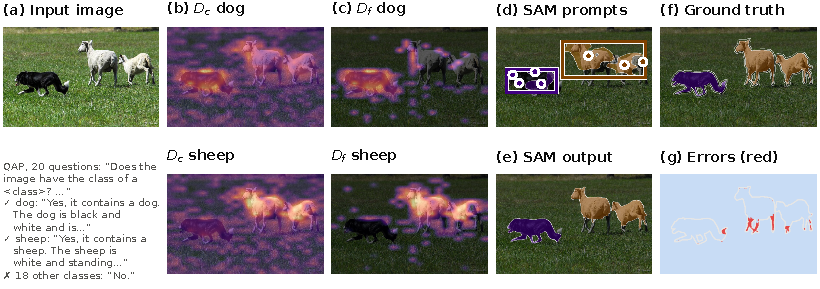
\includegraphics[width=\linewidth]{f_pipeline.pdf}
  \caption{\textbf{The \method{} pipeline on a real VOC validation image, with our implementation's
  intermediate outputs.} (a) LLaVA is asked one yes/no question per class; classes answered ``yes''
  are kept (verbatim answers shown). (b) For each kept class, the cosine similarity between the
  class-name token's hidden state and every image token (layers 7--13) gives a $24\times24$ response
  map $D_c$. (c) Thresholding and a union with description-to-image attention give the reliable map
  $D_f$. (d) Competition with a background level and CLIP prototypes gives a coarse mask, from which
  SAM receives positive points (dots), a box, and the other classes' points as negatives. (e) SAM's
  output after three refinement rounds. (f) Ground truth. (g) Pixel errors. The image was selected
  by a fixed rule (two GT classes, both recognised, per-image mIoU in the 70--80th percentile).}
  \label{fig:pipeline}
\end{figure}

\section{Introduction}
\label{sec:intro}
Open-vocabulary semantic segmentation assigns every pixel to one of a set of class names chosen at
test time. Most strong systems are trained on pixel-level labels or on large image--text corpora with
dense objectives~\citep{li2022lseg,ghiasi2022openseg,liang2023ovseg,xu2022groupvit,cha2023tcl}. A
training-free alternative asks whether the semantic and spatial knowledge already present in frozen
models is enough. \method{}~\citep{zhang2026prior} answers this with two frozen models:
LLaVA~\citep{liu2023llava,liu2024improved} supplies \emph{what} is in the image and a coarse
\emph{where}, and SAM~\citep{kirillov2023sam} supplies precise boundaries (Figure~\ref{fig:pipeline}).
The paper reports 68.0 mIoU on PASCAL VOC with no segmentation training.

A training-free pipeline has many coupled design choices (token positions, layers, thresholds,
prompt construction), and a single final score cannot show which of them carry the result. We
therefore reproduce the method and then take its error apart. We ask four questions:
\begin{enumerate}[label=\textbf{Q\arabic*.}]
  \item Does the published result reproduce in an independent implementation, and how close is the
        authors' own released code?
  \item Which design decisions matter, and where does the released code differ from the paper text?
  \item Does the prior transfer to other VLMs (LLaVA-1.6, Qwen2.5-VL) and to COCO-Object?
  \item Is the remaining error caused by recognition (which classes), by the prior (where), or by SAM
        (boundaries)?
\end{enumerate}

\paragraph{Contributions.} This is a reproduction and analysis study. We do not propose a new
segmentation method, and our implementation does not beat the original.
\begin{itemize}
  \item \textbf{A checked reproduction.} We provide an independent Transformers implementation that
        agrees with the released code per image (Pearson $r=\agreeR$, Section~\ref{sec:repro}), plus
        three implementation facts that are not in the paper text and are needed to reproduce it
        (Table~\ref{tab:diffs}). One of them, the position at which the class token is read, is
        worth 17 points.
  \item \textbf{A decomposition of the error} into recognition, prior coverage, and refinement,
        using oracle-recognition and maps-only controls on VOC and COCO, per class and per object size
        (Section~\ref{sec:errors}).
  \item \textbf{Transfer results} for three further VLMs and a second dataset
        (Section~\ref{sec:transfer}), together with a layer study that separates map quality from
        prompt quality (Section~\ref{sec:layers}).
  \item \textbf{Negative results.} We report eleven improvement attempts, chosen on a separate tuning
        split, none of which transferred to validation (Section~\ref{sec:attempts}).
\end{itemize}

\section{Related work}
\label{sec:related}
\paragraph{Open-vocabulary segmentation with training.} LSeg~\citep{li2022lseg},
OpenSeg~\citep{ghiasi2022openseg} and OVSeg~\citep{liang2023ovseg} align pixel or region features with
text embeddings using segmentation or grounding supervision. GroupViT~\citep{xu2022groupvit} and
TCL~\citep{cha2023tcl} learn grouping from image--text pairs only. These methods train a dense head;
\method{} trains nothing.

\paragraph{Training-free segmentation from CLIP.} MaskCLIP~\citep{zhou2022maskclip},
SCLIP~\citep{wang2024sclip} and ProxyCLIP~\citep{lan2024proxyclip} modify the attention of a frozen
CLIP~\citep{radford2021clip} vision encoder to obtain dense patch--text similarities. They rely on the
contrastive embedding space. \method{} instead reads spatial evidence from the \emph{language model}
inside a multimodal LLM, and uses SAM for boundaries.

\paragraph{Multimodal LLMs for segmentation.} LISA~\citep{lai2024lisa} and related models add a mask
decoder to an MLLM and fine-tune it for segmentation. \method{} keeps LLaVA frozen and treats its
hidden states as a prior. This makes it a useful probe of how much spatial information an
instruction-tuned VLM retains internally.

\paragraph{Reproducibility.} Independent re-implementations often reveal undocumented choices that
matter~\citep{pineau2021improving}; we compare paper text, released code and our implementation under
one protocol.

\section{Method: \method{} and our implementation}
\label{sec:method}
Let $I$ be an image and $\mathcal{C}$ a list of candidate class names (20 for VOC, 80 for COCO).

\paragraph{Question--answer prompting (QAP).} For each $c\in\mathcal{C}$, LLaVA receives the image and
the query ``\emph{Does the image have the class of a $c$? Answer yes or no for this question. If no,
just say `No.' If yes, the answer has to be two sentences, the first sentence is `yes, it contains a
$c$.' the second sentence is to describe the $c$.}'' A class is kept if the greedy answer contains
``yes''. A ``yes'' answer also produces the class-name token and a short description, which the next
two steps use.

\paragraph{Text--visual response.} Let $h^{l}_{c}$ be the hidden state of the class-name token in the
answer at language-model layer $l$, and $h^{l}_{i}$ the hidden state of image token $i$ (576 tokens,
a $24\times24$ grid for LLaVA-1.5). The response map averages cosine similarities over layers $L$
(hidden-state indices 7--13 in the released code):
\begin{equation}
  D_c(i)=\frac{1}{|L|}\sum_{l\in L}\frac{\langle h^l_c, h^l_i\rangle}{\lVert h^l_c\rVert\,\lVert h^l_i\rVert}.
\end{equation}
\paragraph{Reliable map and background.} $D_c$ is thresholded at $\tau_c=\min(\alpha\max_i D_c(i),\beta)$
with $\alpha=0.75$, $\beta=0.19$. Separately, the attention from the description tokens to the image
tokens is averaged over the 30 lowest-entropy (layer, head) pairs and binarised at its mean, giving
$M_A$. The reliable map $D_f$ keeps $D_c$ where the threshold mask \emph{or} $M_A$ is on. Each pixel
then goes to $\arg\max_c D_f$ if that value exceeds a global background level
$\min(\alpha\max_{c,i}D_f,\beta)$, and otherwise to background.

\paragraph{Prototype refinement and SAM.} CLIP patch features (layer $-2$) are averaged inside each
class region to form prototypes, and pixels whose nearest prototype disagrees are removed. The
refined region of each class yields positive points (centres of eroded components), a bounding box,
and, as negative points, the positive points of the other classes. SAM ViT-H is prompted three
times, each time also receiving its previous mask logits. Overlapping masks fall back to LLaVA's
argmax map.

\begin{table}[t]
  \centering
  \caption{\textbf{Implementation facts needed to reproduce \method{}.} The first two are where the
  released code differs from the paper text; the last is an indexing detail stated in neither.
  Effects are measured on VOC val with our implementation (tuning split where marked).}
  \label{tab:diffs}
  \small
  \begin{tabular}{p{3.2cm}p{2.6cm}p{4.2cm}r}
    \toprule
    Component & Paper text & Released code (used here) & Paper version\\
    \midrule
    Combining $D_c$ with $M_A$ & product $D\cdot M_A$ & union of threshold mask and $M_A$ & $-4.23$ (val)\\
    SAM refinement & single prompt & 3 rounds, previous mask logits fed back & $-3.01$ (tuning)\\
    Class-token hidden state & not specified & read \emph{at} the class-name token; one position earlier
      (a literal port of the generate()-based indexing) & $-17.27$ (val)\\
    \bottomrule
  \end{tabular}
\end{table}

\paragraph{Our implementation.} We use Hugging Face Transformers checkpoints
(\texttt{llava-hf/llava-1.5-7b-hf}, fp16) and the official SAM ViT-H weights. The pipeline has three
separate stages. \emph{Trace} runs LLaVA once per image and caches the answers, $P(\text{yes})$,
per-layer response maps, attention, and CLIP features. \emph{Segment} reruns only the SAM stage, so
each ablation costs minutes instead of hours. \emph{Evaluate} accumulates a confusion matrix. Every
setting in this report is a configuration of the same code. Table~\ref{tab:diffs} lists what we had
to learn from the released code. The class-token position was the hardest to find: our first port
read the state one position early and scored 48.6.

\section{Experimental setup}
\label{sec:setup}
\paragraph{Datasets.}
\textbf{PASCAL VOC 2012}~\citep{everingham2010pascal} has 20 object classes plus background, with
pixel-level masks drawn by the VOC annotators. Object boundaries are marked as a 5-pixel \emph{void}
band (label 255), which is ignored in scoring. We use the official segmentation \texttt{val} split
(1,449 images, archive SHA-256 verified) only for final numbers. Design choices were made on a
separate \textbf{tuning split} of 200 images drawn from VOC \texttt{train} with seed 0, which shares no
images with val. \textbf{COCO-Object} is the standard training-free benchmark derived from COCO
2017~\citep{lin2014coco} \texttt{val} (5,000 images): the 80 ``thing'' categories plus background. We
build it from the official instance annotations by painting every instance mask, crowd regions
included, in annotation order; pixels with no instance are background. This follows the protocol of
GroupViT/TCL/SCLIP-style evaluations, but small differences in conversion scripts across papers mean
that COCO numbers from different papers are not strictly comparable.

\paragraph{Models.} LLaVA-1.5-7B~\citep{liu2024improved} (the paper's model), LLaVA-1.6
(LLaVA-NeXT~\citep{liu2024llavanext}) with Vicuna-7B~\citep{chiang2023vicuna} and
Mistral-7B~\citep{jiang2023mistral} language models, and Qwen2.5-VL-7B~\citep{bai2025qwen25vl}, all
frozen. LLaVA-1.6 uses its own chat templates and only the base-resolution $24\times24$ image tokens
for the maps. For Mistral, $\beta$ was set to 0.16 on the tuning split (Appendix~\ref{app:tuning}).
SAM is ViT-H~\citep{kirillov2023sam} in all runs.

\paragraph{Protocol and metric.} We report VOC21 mIoU (VOC) or 81-class mIoU (COCO). Intersections
and unions are accumulated over the whole split, as in mmsegmentation, and void pixels are ignored.
Confidence intervals are 95\% percentile bootstrap intervals over images (1,000 resamples); paired
differences resample the same images for both systems~\citep{efron1994bootstrap}. Two diagnostic
controls are never presented as results. \emph{Maps only} scores LLaVA's coarse label map without
SAM. \emph{Oracle recognition} replaces the QAP answer with the ground-truth class list and keeps
everything else fixed. The released code was run in its pinned environment (PyTorch 2.1.2,
Transformers 4.37, original \texttt{liuhaotian/llava-v1.5-7b} weights) on the same images and scored
by our evaluator. All runs used one NVIDIA A30 (24\,GB); total compute is in
Appendix~\ref{app:compute}.

\section{Results}
\subsection{Reproduction (Q1)}
\label{sec:repro}
\begin{figure}[t]
  \centering
  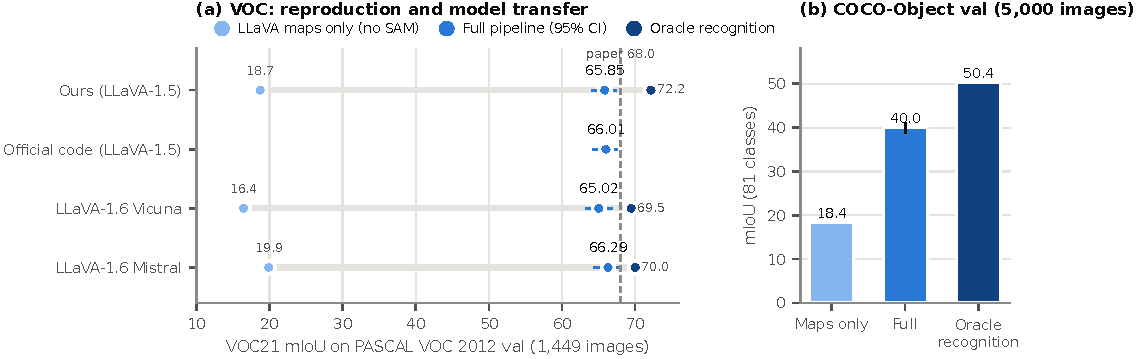
\includegraphics[width=\linewidth]{f_main.pdf}
  \caption{\textbf{Main results.} Each row shows LLaVA's maps without SAM (light), the full pipeline
  with its 95\% bootstrap CI (mid), and the pipeline with the true class list (dark; diagnostic
  only). (a) VOC val: our implementation, the authors' released code, and two LLaVA-1.6 models used
  without retuning. Dashed line: the paper's 68.0. (b) COCO-Object val with LLaVA-1.5.}
  \label{fig:main}
\end{figure}

Our implementation obtains \textbf{\miouOurs{}} mIoU on VOC val (CI \ciOurs{}) and the released code
obtains \textbf{\miouOfficial{}} (CI \ciOfficial{}). The paired difference is \dOfficial{} points
(CI \dciOfficial{}), so the two implementations are statistically indistinguishable. Both are about
2 points below the paper's 68.0 (Figure~\ref{fig:main}a). Per image they agree closely
(Figure~\ref{fig:agreement}, Appendix): Pearson $r=\agreeR$, and \agreeWithin\% of images are
within 5 points. Because the authors' own code in its pinned environment also lands at 66.0, the
gap to the paper is not caused by our port, by the Hugging Face checkpoint conversion, or by newer
library versions. One explanation we cannot test is the class-name file used for the paper, which is
not public: on the tuning split, natural names (``potted plant'' instead of ``pottedplant'') cost 1.4
points, so the vocabulary alone moves results by this order.

\subsection{What matters inside the pipeline (Q2)}
\label{sec:ablation}
\begin{figure}[t]
  \centering
  \begin{minipage}[t]{0.49\linewidth}
    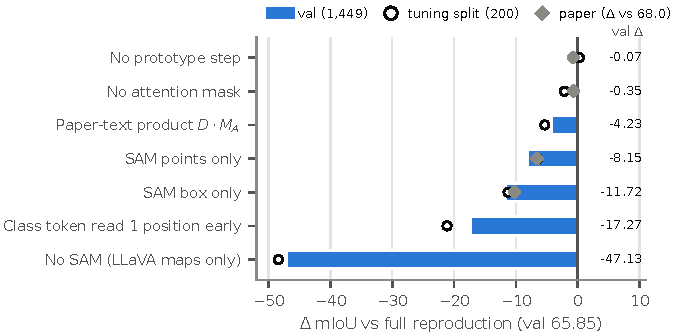
\includegraphics[width=\linewidth]{f_ablation.pdf}
    \caption{\textbf{Ablations} (Δ vs the full reproduction). Bars: VOC val. Circles: tuning split.
    Diamonds: the paper's ablations relative to its 68.0. The trends match the paper (box + points
    $>$ points $>$ box; attention helps; prototypes matter little).}
    \label{fig:ablation}
  \end{minipage}\hfill
  \begin{minipage}[t]{0.49\linewidth}
    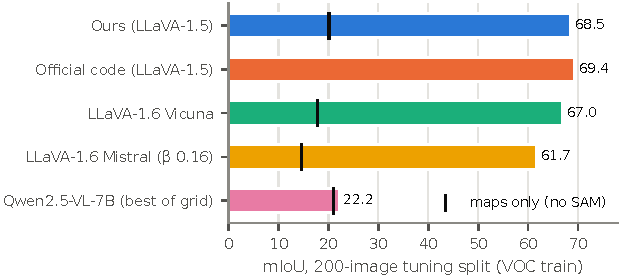
\includegraphics[width=\linewidth]{f_models_dev.pdf}
    \caption{\textbf{Five systems on the 200-image tuning split.} Bars: full pipeline. Ticks: maps
    only. All LLaVA variants work with the paper's settings (Mistral with $\beta=0.16$), and Qwen2.5-VL
    does not, even after an 18-setting $(\alpha,\beta)$ grid and hidden-state centring.}
    \label{fig:models_dev}
  \end{minipage}
\end{figure}

Figure~\ref{fig:ablation} reproduces the paper's ablation directions. SAM is the largest single
component: the coarse LLaVA map alone scores 18.7, and SAM with points and a box adds 47 points.
Points and box are complementary (points only $-8.2$, box only $-11.7$). The attention mask
($-0.35$ without it) and the prototype step ($+0.07$ without it) matter much less on val than in the
paper ($-0.7$ each). Two choices from Table~\ref{tab:diffs} matter far more than any listed in the
paper: the union-versus-product combination ($-4.2$) and, above all, the class-token position
($-17.3$). The response map is sensitive to which token's state is read. The neighbouring token
(``a'') carries a generic, non-localised representation.

\subsection{Transfer to other VLMs and to COCO (Q3)}
\label{sec:transfer}
\paragraph{LLaVA-1.6.} Both LLaVA-1.6 models work without retuning
(Figure~\ref{fig:main}a): Vicuna \miouVic{} (paired Δ vs LLaVA-1.5 \dVic{}, CI \dciVic{}) and
Mistral \miouMis{} (Δ \dMis{}, CI \dciMis{}). Neither difference is significant. The \emph{per-class}
picture differs much more than the averages (Figure~\ref{fig:per_class}). Mistral more than doubles
\textbf{person} IoU (40 vs 19), the weakest class for LLaVA-1.5, and improves chair and sofa, but loses
on boat, TV/monitor and aeroplane. Its recognition is more conservative (precision \qPMis{}, recall
\qRMis{}, vs \qPOurs{}/\qROurs{} for LLaVA-1.5, Figure~\ref{fig:recognition}b), so it removes false
``yes'' answers but misses more present classes.

\paragraph{Qwen2.5-VL.} With the same procedure, Qwen2.5-VL reaches only 22.2 on the tuning split, at
the level of its maps alone (Figure~\ref{fig:models_dev}). Its image-token hidden states are strongly
anisotropic: the median cosine between class and image tokens is 0.47, against 0.09 for LLaVA-1.5, so
every location looks similar to every class. Removing the mean image-token state (centring) did not
help (best 17.0), and neither did an 18-setting $(\alpha,\beta)$ grid. We conclude that the mechanism
depends on the LLaVA family's representation geometry. We do not claim it fails for every other
architecture.

\paragraph{COCO-Object.} On 5,000 COCO images with 80 classes, the pipeline reaches \miouCoco{} (CI
\ciCoco{}); SAM adds 21.6 points over the maps alone (Figure~\ref{fig:main}b). Recognition is the
larger limit here: the oracle class list adds \dCocoOracle{} points (CI \dciCocoOracle{}), against
\dOracle{} on VOC. Per class, the oracle gain tracks low recognition \emph{precision} (Pearson
$r=\cocoGainPrecR{}$; with recall $r=\cocoGainRecR{}$, Figure~\ref{fig:coco}a), so on COCO the oracle
mostly removes false ``yes'' answers. Toaster is the extreme case: LLaVA affirmed it 77 times for 8
true occurrences. Person is again among the weakest classes (Figure~\ref{fig:coco}b), as on VOC.
Qualitative examples are in Figure~\ref{fig:coco_examples} (Appendix).

\begin{figure}[t]
  \centering
  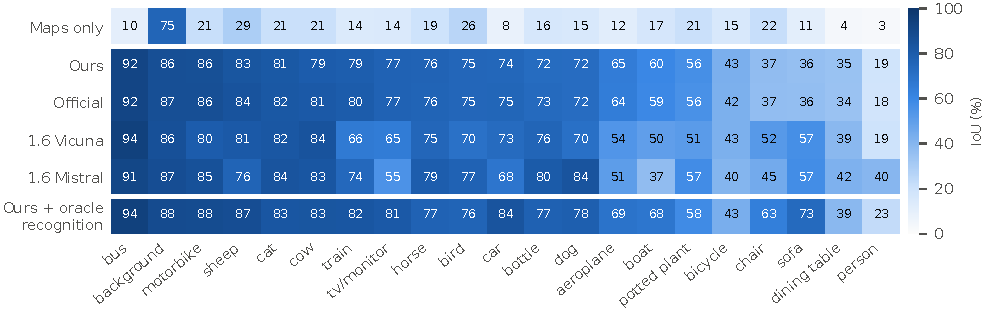
\includegraphics[width=\linewidth]{f_per_class.pdf}
  \caption{\textbf{Per-class IoU on VOC val} (classes sorted by our IoU). The two LLaVA-1.5
  implementations are almost identical per class. LLaVA-1.6 Mistral gains on person, chair and sofa
  and loses on boat and TV/monitor. Person stays the weakest class for LLaVA-1.5 even with oracle
  recognition (23), so its problem is the prior, not recognition.}
  \label{fig:per_class}
\end{figure}

\subsection{Where the spatial information sits: a layer study}
\label{sec:layers}
\begin{figure}[t]
  \centering
  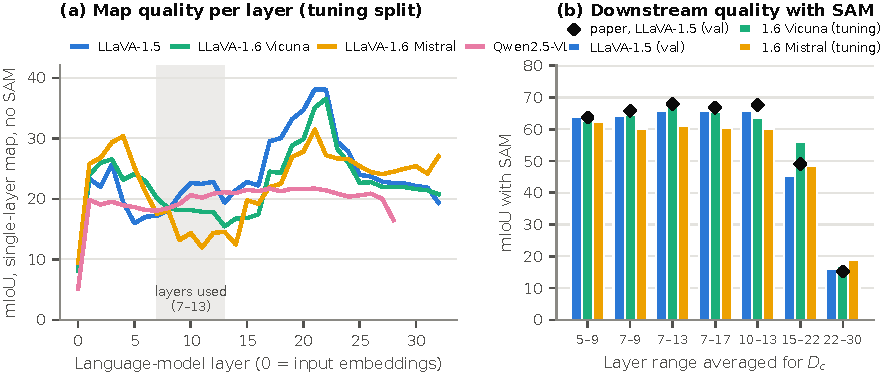
\includegraphics[width=\linewidth]{f_layers.pdf}
  \caption{\textbf{Layer study.} (a) mIoU of the maps from a single layer, without SAM, for four VLMs
  (tuning split). Stand-alone map quality peaks at layers 20--22 for LLaVA-1.5 and LLaVA-1.6 Vicuna.
  (b) With SAM, the paper's layer ranges reproduce on val (diamonds: the paper's Table~3). Middle
  ranges are best, and the deep ranges that give the best maps collapse. Per-layer maps of one image
  are in Figure~\ref{fig:layer_maps} (Appendix).}
  \label{fig:layers}
\end{figure}

The layer used to read $D_c$ matters, and the best layer depends on what the map is used for
(Figure~\ref{fig:layers}). As stand-alone segmentations, single-layer maps improve sharply after
layer 16 and peak at layers 21--22 (37.5 on val for LLaVA-1.5). As SAM prompts, the same deep ranges
are the worst: 15--22 gives 45.5 and 22--30 gives 16.1, against 65.9 for 7--13. The reason is seed
precision. Middle-layer maps mark only 5\% of pixels, and 79\% of those are correct, so SAM receives
reliable points inside the object. Layers 15--22 mark larger, less precise regions (precision 0.50),
and the resulting SAM masks cover 43\% of pixels against 27\% true foreground. Both LLaVA-1.6 models
follow the same pattern. Qwen2.5-VL's curve is flat at about 20 for every layer, which matches its
failure above. The practical lesson for training-free pipelines is to choose layers by the quality of
the downstream prompts, not by how good the maps look.

\section{Error analysis (Q4)}
\label{sec:errors}
\begin{figure}[t]
  \centering
  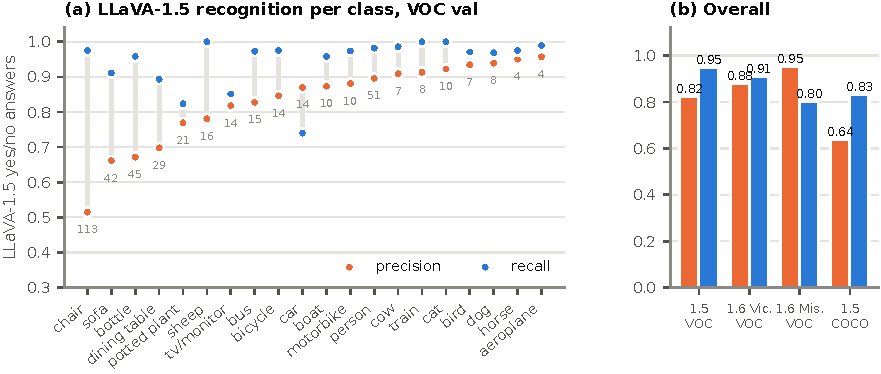
\includegraphics[width=0.92\linewidth]{f_recognition.pdf}
  \caption{\textbf{Recognition (QAP) errors.} (a) Per-class precision and recall of LLaVA-1.5's
  yes/no answers on VOC val; grey numbers count false ``yes'' answers. Precision is low for chair,
  dining table, sofa and bottle, which co-occur with other furniture and indoor scenes. Grey numbers:
  count of false ``yes'' answers. (b) Overall precision and recall per model and dataset.}
  \label{fig:recognition}
\end{figure}

\paragraph{Recognition.} Over $1{,}449\times20$ VOC questions, LLaVA-1.5 answers ``yes'' wrongly
\qFPOurs{} times and ``no'' wrongly \qFNOurs{} times (precision \qPOurs{}, recall \qROurs{};
Figure~\ref{fig:recognition}). False ``yes'' answers concentrate on chair, dining table, sofa and
bottle: in an indoor scene, LLaVA tends to affirm furniture that is plausible but absent. A false
``yes'' is costly, because the class then competes for pixels and is passed to SAM. On COCO, with 80
questions per image, false ``yes'' answers dominate: precision drops to \qPCoco{} (\qFPCoco{} false
``yes'' against \qFNCoco{} misses; recall \qRCoco{}).

\begin{figure}[t]
  \centering
  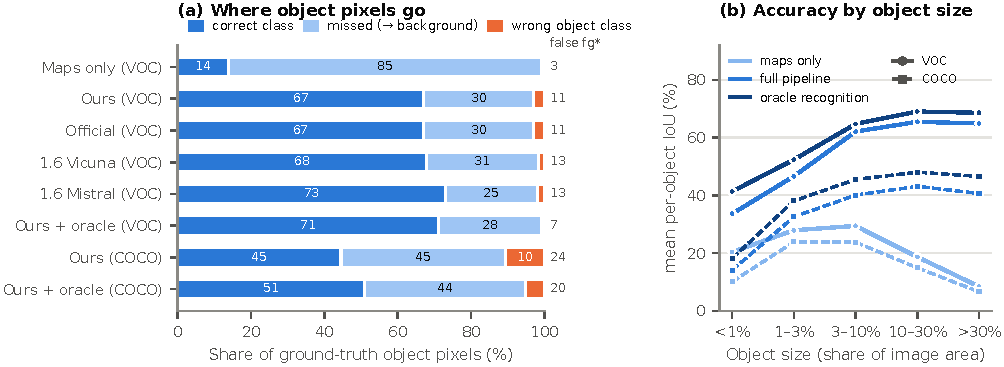
\includegraphics[width=0.92\linewidth]{f_errors.pdf}
  \caption{\textbf{Where the error comes from.} (a) Fate of every ground-truth object pixel: correctly
  labelled, left as background, or given another object class. The number to the right is the count
  of background pixels labelled as an object, per 100 object pixels. (b) Mean per-object IoU by
  object size (share of image area) for maps only, the full pipeline, and oracle recognition, on VOC
  (solid) and COCO (dashed).}
  \label{fig:errors}
\end{figure}

\paragraph{Missed pixels, not confused classes.} Figure~\ref{fig:errors}a follows every ground-truth
object pixel. With LLaVA-1.5 on VOC, \eCorrectOurs\% are labelled correctly, \eBgOurs\% are left as
background, and only \eWrongOurs\% receive another object class. Oracle recognition removes most of
the wrong-class share (to \eWrongOursOracle\%) but leaves the background share almost unchanged
(\eBgOursOracle\%). The dominant failure is therefore an \emph{incomplete prior}: the object is
recognised, but part of it is never prompted. On COCO the background share is larger
(\eBgCoco\%).

\paragraph{Object size.} Accuracy rises with object size up to objects of 10--30\% of the image and
then flattens (Figure~\ref{fig:errors}b). Small objects ($<$1\% of the image; \sizeCocoSmallShare\%
of COCO objects) reach only \sizeCocoSmall{} IoU on COCO (\sizeVocSmall{} on VOC): at a $24\times24$
grid, each token covers about 0.17\% of the image, so a small object occupies one or two tokens and
the prior often misses it. For large objects, the maps alone collapse (\sizeVocCoarseLarge{} IoU on VOC
for objects above 30\% of the image, against \sizeVocLarge{} with SAM): the response concentrates on the
most distinctive part, such as a face or a wheel. SAM's box usually recovers the full extent, and
close-ups where it does not are the person failures discussed below.

\begin{figure}[t]
  \centering
  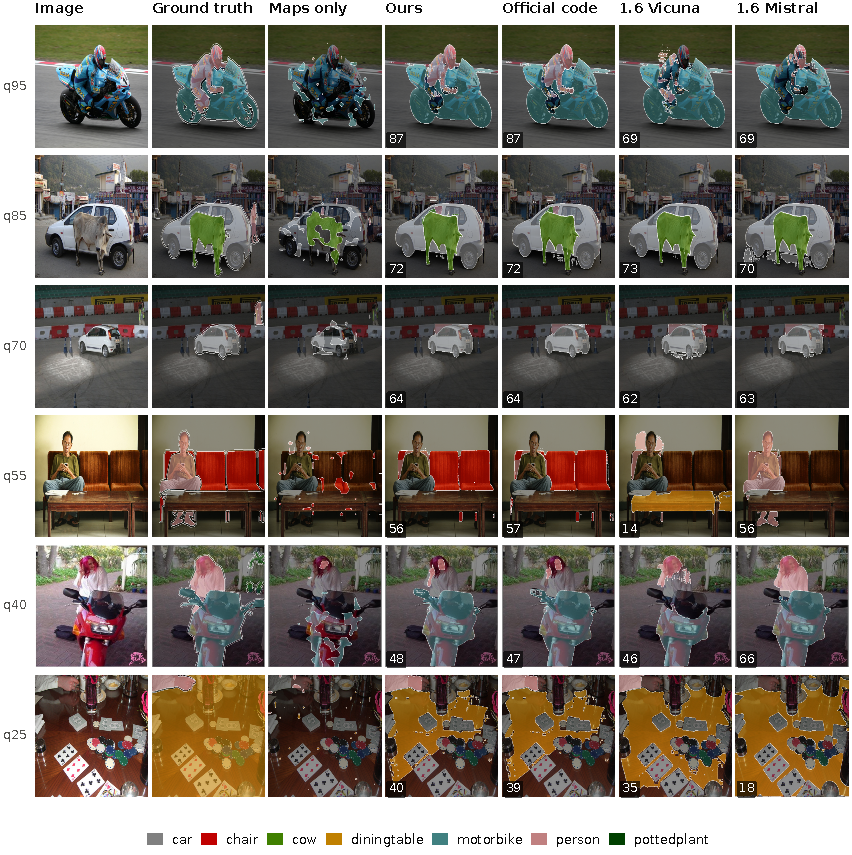
\includegraphics[width=0.8\linewidth]{f_qualitative.pdf}
  \caption{\textbf{Qualitative comparison on VOC val.} Rows are images at fixed quantiles (95th to
  25th) of our per-image mIoU, among images with at least two classes, so the rows span good to
  below-median cases rather than hand-picked successes. Numbers: per-image mIoU. ``LLaVA maps only''
  is the coarse prior before SAM.}
  \label{fig:qualitative}
\end{figure}

\paragraph{Qualitative evidence.} Figure~\ref{fig:qualitative} compares all systems on six images at
fixed quantiles, and Figure~\ref{fig:failures} shows one example of each failure type with LLaVA's
verbatim answer. (a) In close-ups, the person response covers the face or skin. Over all of VOC
val, 78\% of person pixels end up as background, and 84\% in the 49 images where a person covers more
than 45\% of the frame. (b) A missed class has no map at all, so nothing can recover it.
(c) A false ``yes'' produces a confident description of an object that is not there, and SAM then
segments whatever region the map points to. (d) Small objects fall between grid cells. These four
types correspond to the three quantitative findings above: recognition, prior coverage, and
resolution.

\begin{figure}[t]
  \centering
  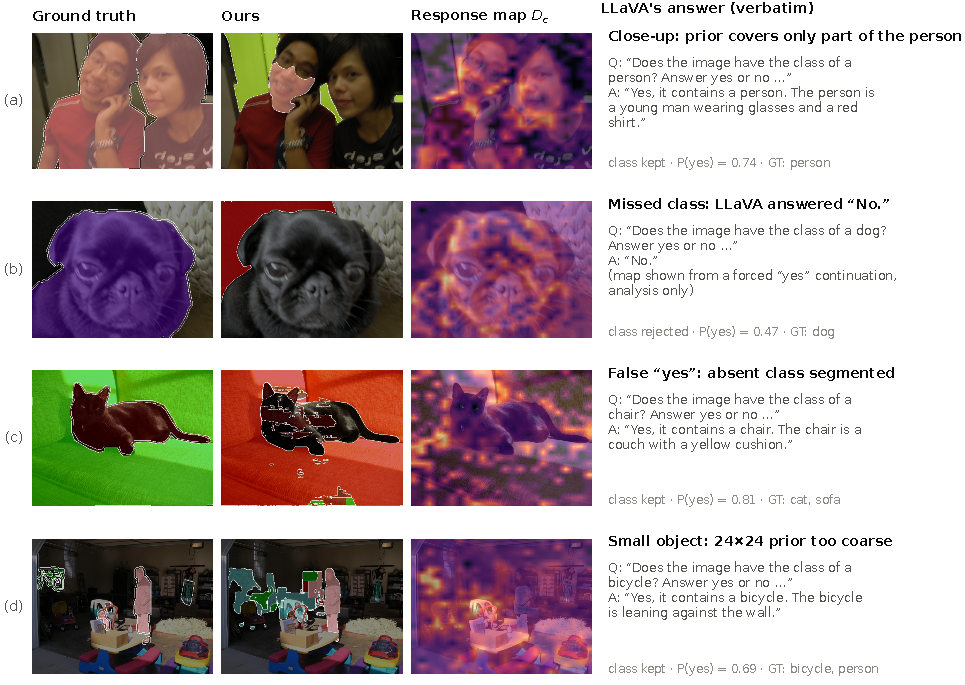
\includegraphics[width=0.82\linewidth]{f_failures.pdf}
  \caption{\textbf{Failure types} with LLaVA-1.5's verbatim answers, chosen by fixed rules
  (Appendix~\ref{app:selection}). (a) Close-up: the prior and SAM cover one face. (b) Missed class:
  LLaVA answers ``No.'' to a dog filling the frame ($P(\text{yes})=0.47$). (c) False ``yes'': LLaVA
  calls the sofa ``a chair \ldots{} a couch with a yellow cushion'', and the pipeline labels it chair.
  (d) A small bicycle that is recognised but falls between grid cells.}
  \label{fig:failures}
\end{figure}

\section{What did not work}
\label{sec:attempts}
\begin{wrapfigure}{r}{0.5\linewidth}
  \vspace{-12pt}
  \centering
  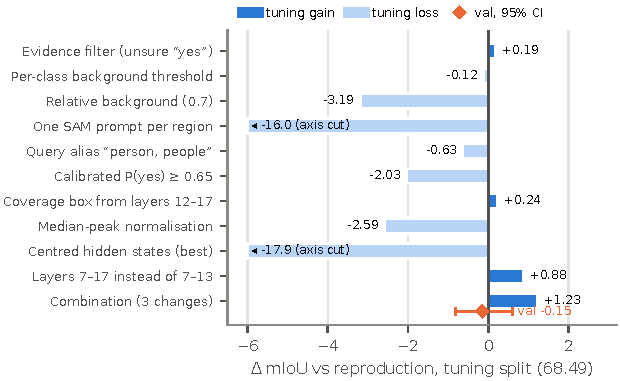
\includegraphics[width=\linewidth]{f_attempts.pdf}
  \caption{\textbf{Improvement attempts}, each targeting a measured error source, on the tuning
  split. The only gain above noise (the combination, +1.23) was frozen and run once on val, where it
  scored \dCombo{} (CI \dciCombo{}).}
  \label{fig:attempts}
  \vspace{-10pt}
\end{wrapfigure}
We tried to fix each error source found above, choosing on the tuning split and keeping val untouched
(Figure~\ref{fig:attempts}). For \emph{recognition}, we tested an evidence filter that drops unsure
``yes'' classes with tiny maps, calibrated thresholds on $P(\text{yes})$, and a query alias (``person,
people''). For the \emph{incomplete prior}, we tested per-class background levels, relative
backgrounds, a SAM box extended to the deep-layer region, and one SAM prompt per connected region.
For \emph{representation}, we tested map normalisation and hidden-state centring. Per-class
backgrounds raised person IoU by 13.8 on the tuning split but cost other classes as much. One prompt
per region was much worse, because the LLaVA region is fragmented \emph{within} a single object. The
only candidate above noise was a combination of three small changes (+1.23 on tuning, CI
$[-0.5, +3.5]$). We froze it and ran it once on val, where it scored \dCombo{} (CI \dciCombo{}). The
tuning gain was sampling noise from 200 images, so our final number is the plain reproduction.

\section{Discussion and limitations}
\label{sec:discussion}
\paragraph{What the results support.} (1) The method reproduces: two independent implementations
agree per image, and the remaining gap to the paper is shared by the authors' code. (2) It transfers
within the LLaVA family and to COCO, but not to Qwen2.5-VL. (3) SAM does most of the
boundary work, so the useful output of LLaVA is a \emph{precise seed} rather than a complete map.

\paragraph{Limitations.} We use one SAM variant and 7B-scale VLMs only. The Qwen2.5-VL result comes
from the 200-image tuning split and one family of fixes, so it shows that the method does not
transfer \emph{as is}, not that it cannot be adapted. We did not evaluate PASCAL Context, ADE20K or
COCO-Stuff (dataset use was limited to VOC and COCO), so we cannot speak to stuff classes or
vocabularies of 150+ classes. The oracle numbers are diagnostic upper bounds, not methods. The
layer-study and LLaVA-1.6 tuning numbers use 200 images, and differences below about 1.5 points there
are within noise (Section~\ref{sec:attempts}).

\paragraph{Broader impact.} Training-free segmentation makes masks for new classes cheap, but it
inherits the VLM's recognition errors and biases; the confident false descriptions in
Figure~\ref{fig:failures}c show that an MLLM's ``yes'' is not evidence on its own. We use public
benchmarks only.

\section{Conclusion}
Our reproduction of \method{} (\miouOurs{} VOC mIoU) matches the released code (\miouOfficial{}). The
remaining error comes from LLaVA's yes/no recognition (6.3 points on VOC, 10.4 on COCO) and from priors
that are incomplete on large objects and too coarse for small ones; SAM carries the boundaries.

\small
\bibliographystyle{plainnat}
\begin{thebibliography}{99}
\bibitem[Bai et~al.(2025)]{bai2025qwen25vl} S.~Bai, K.~Chen, X.~Liu, et~al. Qwen2.5-VL technical report. \emph{arXiv:2502.13923}, 2025.
\bibitem[Cha et~al.(2023)]{cha2023tcl} J.~Cha, J.~Mun, and B.~Roh. Learning to generate text-grounded mask for open-world semantic segmentation from only image-text pairs. In \emph{CVPR}, 2023.
\bibitem[Chiang et~al.(2023)]{chiang2023vicuna} W.-L.~Chiang, Z.~Li, Z.~Lin, et~al. Vicuna: An open-source chatbot impressing GPT-4 with 90\%* ChatGPT quality. LMSYS blog, 2023.
\bibitem[Efron and Tibshirani(1994)]{efron1994bootstrap} B.~Efron and R.~J.~Tibshirani. \emph{An Introduction to the Bootstrap}. Chapman \& Hall/CRC, 1994.
\bibitem[Everingham et~al.(2010)]{everingham2010pascal} M.~Everingham, L.~Van~Gool, C.~K.~I.~Williams, J.~Winn, and A.~Zisserman. The PASCAL visual object classes (VOC) challenge. \emph{IJCV}, 88(2):303--338, 2010.
\bibitem[Ghiasi et~al.(2022)]{ghiasi2022openseg} G.~Ghiasi, X.~Gu, Y.~Cui, and T.-Y.~Lin. Scaling open-vocabulary image segmentation with image-level labels. In \emph{ECCV}, 2022.
\bibitem[Jiang et~al.(2023)]{jiang2023mistral} A.~Q.~Jiang, A.~Sablayrolles, A.~Mensch, et~al. Mistral 7B. \emph{arXiv:2310.06825}, 2023.
\bibitem[Kirillov et~al.(2023)]{kirillov2023sam} A.~Kirillov, E.~Mintun, N.~Ravi, et~al. Segment anything. In \emph{ICCV}, 2023.
\bibitem[Lai et~al.(2024)]{lai2024lisa} X.~Lai, Z.~Tian, Y.~Chen, Y.~Li, Y.~Yuan, S.~Liu, and J.~Jia. LISA: Reasoning segmentation via large language model. In \emph{CVPR}, 2024.
\bibitem[Lan et~al.(2024)]{lan2024proxyclip} M.~Lan, C.~Chen, Y.~Ke, X.~Wang, L.~Feng, and W.~Zhang. ProxyCLIP: Proxy attention improves CLIP for open-vocabulary segmentation. In \emph{ECCV}, 2024.
\bibitem[Li et~al.(2022)]{li2022lseg} B.~Li, K.~Q.~Weinberger, S.~Belongie, V.~Koltun, and R.~Ranftl. Language-driven semantic segmentation. In \emph{ICLR}, 2022.
\bibitem[Liang et~al.(2023)]{liang2023ovseg} F.~Liang, B.~Wu, X.~Dai, et~al. Open-vocabulary semantic segmentation with mask-adapted CLIP. In \emph{CVPR}, 2023.
\bibitem[Lin et~al.(2014)]{lin2014coco} T.-Y.~Lin, M.~Maire, S.~Belongie, et~al. Microsoft COCO: Common objects in context. In \emph{ECCV}, 2014.
\bibitem[Liu et~al.(2023)]{liu2023llava} H.~Liu, C.~Li, Q.~Wu, and Y.~J.~Lee. Visual instruction tuning. In \emph{NeurIPS}, 2023.
\bibitem[Liu et~al.(2024a)]{liu2024improved} H.~Liu, C.~Li, Y.~Li, and Y.~J.~Lee. Improved baselines with visual instruction tuning. In \emph{CVPR}, 2024.
\bibitem[Liu et~al.(2024b)]{liu2024llavanext} H.~Liu, C.~Li, Y.~Li, B.~Li, Y.~Zhang, S.~Shen, and Y.~J.~Lee. LLaVA-NeXT: Improved reasoning, OCR, and world knowledge. Blog post, 2024.
\bibitem[Pineau et~al.(2021)]{pineau2021improving} J.~Pineau, P.~Vincent-Lamarre, K.~Sinha, et~al. Improving reproducibility in machine learning research. \emph{JMLR}, 22(164):1--20, 2021.
\bibitem[Radford et~al.(2021)]{radford2021clip} A.~Radford, J.~W.~Kim, C.~Hallacy, et~al. Learning transferable visual models from natural language supervision. In \emph{ICML}, 2021.
\bibitem[Wang et~al.(2024)]{wang2024sclip} F.~Wang, J.~Mei, and A.~Yuille. SCLIP: Rethinking self-attention for dense vision-language inference. In \emph{ECCV}, 2024.
\bibitem[Xu et~al.(2022)]{xu2022groupvit} J.~Xu, S.~De~Mello, S.~Liu, et~al. GroupViT: Semantic segmentation emerges from text supervision. In \emph{CVPR}, 2022.
\bibitem[Zhang et~al.(2026)]{zhang2026prior} Zhang et~al. The power of prior: Training-free open-vocabulary semantic segmentation with LLaVA. In \emph{CVPR}, 2026. Code: \url{https://github.com/zbf1991/FSeg-LLaVA}.
\bibitem[Zhou et~al.(2022)]{zhou2022maskclip} C.~Zhou, C.~C.~Loy, and B.~Dai. Extract free dense labels from CLIP. In \emph{ECCV}, 2022.
\end{thebibliography}
\normalsize

\appendix
\section{Implementation agreement and COCO examples}
\begin{figure}[h]
  \centering
  \begin{minipage}[c]{0.34\linewidth}
    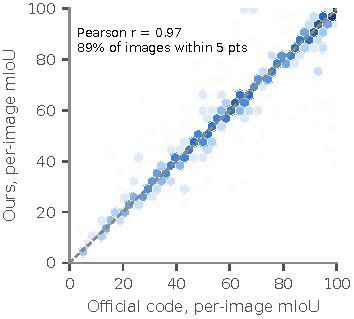
\includegraphics[width=\linewidth]{f_agreement.pdf}
  \end{minipage}\hfill
  \begin{minipage}[c]{0.62\linewidth}
    \caption{\textbf{Per-image agreement between our implementation and the released code} on the
    1,449 VOC val images (hexbin counts; dashed line = equality). Pearson $r=\agreeR$; \agreeWithin\%
    of images are within 5 points. Most remaining disagreement comes from images where one
    implementation keeps a borderline class and the other does not. Different LLaVA weights
    (original vs.\ HF-converted) and fp16 kernels can flip such greedy answers.}
    \label{fig:agreement}
  \end{minipage}
\end{figure}

\begin{figure}[h]
  \centering
  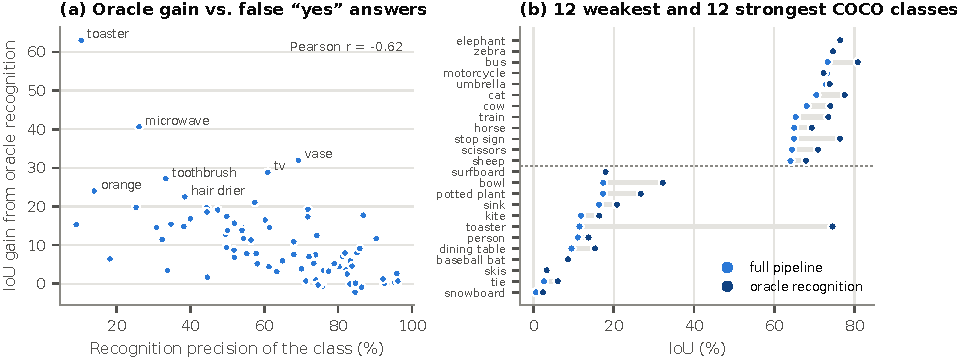
\includegraphics[width=\linewidth]{f_coco_classes.pdf}
  \caption{\textbf{COCO-Object per class.} (a) IoU gain from oracle recognition against the class's
  recognition precision: classes with many false ``yes'' answers gain most. (b) The 12 weakest and 12 strongest
  classes (full pipeline vs.\ oracle recognition).}
  \label{fig:coco}
\end{figure}

\begin{figure}[h]
  \centering
  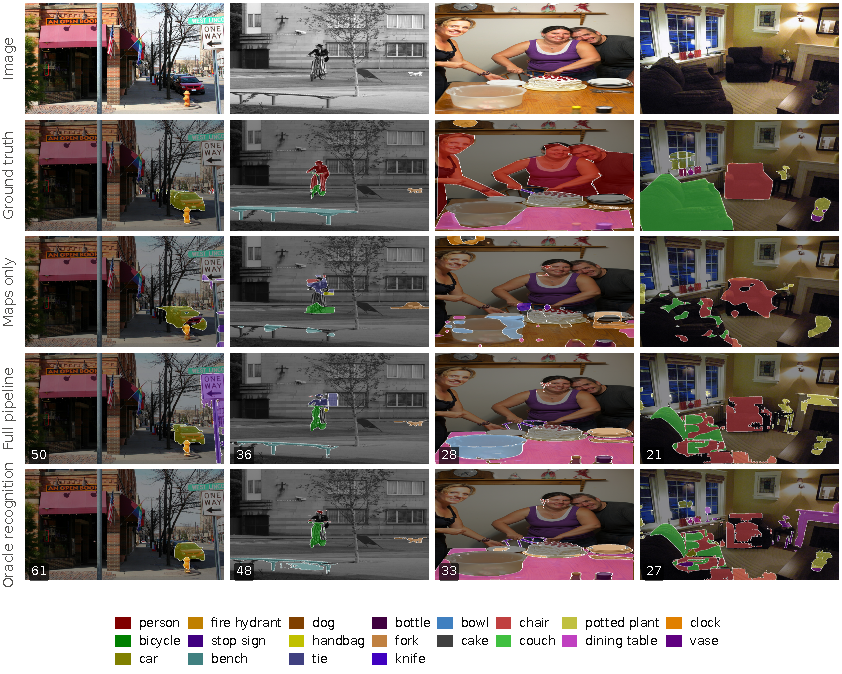
\includegraphics[width=\linewidth]{f_coco_examples.pdf}
  \caption{\textbf{COCO-Object examples} at the 90th, 70th, 50th and 30th percentile of per-image mIoU
  (images with $\geq$3 classes). Numbers: per-image mIoU. Small objects and crowded scenes lose most;
  oracle recognition restores missed classes but not missing extent.}
  \label{fig:coco_examples}
\end{figure}

\begin{figure}[h]
  \centering
  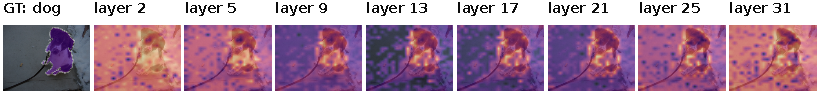
\includegraphics[width=\linewidth]{f_layer_maps.pdf}
  \caption{\textbf{Response map $D_c$ of a single layer, from early to late layers}, for one VOC val
  image (selection rule in Appendix~\ref{app:selection}). Each map is min--max scaled.}
  \label{fig:layer_maps}
\end{figure}

\section{Tuning decisions}
\label{app:tuning}
All decisions used the 200-image tuning split. LLaVA-1.5 keeps the released defaults: $\alpha=0.75$
and $\beta=0.19$ were best among $\alpha\in\{0.65,0.75,0.85\}$ (67.5, 68.5, 67.3) and
$\beta\in\{0.16,0.19,0.22\}$ (65.0, 68.5, 64.3). LLaVA-1.6 Vicuna uses the same values. LLaVA-1.6
Mistral produces lower cosine levels; $\beta\in\{0.13,0.16,0.19,0.22\}$ gave 53.0, 61.7, 61.1 and
61.3, so it uses $\beta=0.16$ on val. Qwen2.5-VL was given a $6\times3$ $(\beta,\alpha)$ grid (best
22.2), all eight layer ranges (14.2--15.8 with SAM), three normalisations, and centred hidden states
(best 17.0). Its best setting is reported in Figure~\ref{fig:models_dev}.

\section{Example selection}
\label{app:selection}
To avoid cherry-picking, every image shown was chosen by a fixed rule, written in the figure script
(\texttt{reports/neurips/make\_figures.py}) and logged with the chosen IDs in
\texttt{data/selection.json}. Figure~\ref{fig:pipeline}: the best-ranked image with two GT classes,
both recognised, and per-image mIoU in the 70--80th percentile. Figure~\ref{fig:layer_maps}: the 4th-best
single-object animal image with 15--35\% area and IoU $\geq0.85$. Figure~\ref{fig:qualitative} and
Figure~\ref{fig:coco_examples}: fixed quantiles of per-image mIoU. Figure~\ref{fig:failures}:
(a) the median-IoU case among person-only images where the person covers $>$45\% of the frame, is
recognised, and has IoU $<$0.3; (b) the largest object whose class LLaVA rejected, with IoU $<$0.05, that
oracle recognition recovers to $\geq$0.7; (c) the largest predicted area of an absent class (every third
val image scanned); (d) the median case among recognised non-person objects below 2\% of the image with
IoU $<$0.2. For a rejected class the map is taken from a forced ``yes'' continuation that the
pipeline itself never uses.

\section{Compute}
\label{app:compute}
\begin{table}[h]
  \centering
  \caption{Wall-clock time of the main jobs on one A30 GPU. LLaVA tracing is the cost; every SAM-only
  ablation then reuses the cache.}
  \label{tab:compute}
  \small
  \begin{tabular}{lrr}
    \toprule
    Job & Images & Time (h:mm)\\
    \midrule
    LLaVA-1.5 trace, VOC val & 1,449 & 2:49\\
    SAM + scoring, 8 VOC val configurations & 1,449 & 1:14\\
    Layer study, VOC val (per-layer traces + 16 configurations) & 1,449 & 6:44\\
    Released code, VOC val (pinned environment) & 1,449 & 3:06\\
    LLaVA-1.6 Vicuna, trace + SAM, VOC val & 1,449 & 4:19\\
    LLaVA-1.6 Mistral, trace + SAM, VOC val & 1,449 & 2:24\\
    LLaVA-1.5, trace + SAM, COCO-Object val & 5,000 & 13:46\\
    \midrule
    All GPU jobs of the project (40, incl. cancelled reruns) & & $\approx$ 48\\
    \bottomrule
  \end{tabular}
\end{table}

\newpage
\section*{NeurIPS Paper Checklist (abridged)}
\small
\begin{enumerate}[leftmargin=*]
\item \textbf{Claims.} Do the abstract and introduction reflect the contributions? \textbf{Yes}: the
  work is framed as a reproduction and analysis; no new state of the art is claimed.
\item \textbf{Limitations.} \textbf{Yes}, Section~\ref{sec:discussion}.
\item \textbf{Theory.} \textbf{NA}: no theoretical results.
\item \textbf{Reproducibility.} \textbf{Yes}: Sections~\ref{sec:method}--\ref{sec:setup},
  Table~\ref{tab:diffs} and Appendix~\ref{app:tuning} give every setting; all numbers and figures are
  regenerated by scripts from saved outputs.
\item \textbf{Open access to data and code.} \textbf{Yes} for data (public benchmarks). The code is in
  the project repository and can be shared on request.
\item \textbf{Experimental details.} \textbf{Yes}: tuning split, frozen val evaluation, Section~\ref{sec:setup}.
\item \textbf{Statistical significance.} \textbf{Yes}: 95\% bootstrap CIs over images and paired
  bootstrap for differences.
\item \textbf{Compute resources.} \textbf{Yes}, Appendix~\ref{app:compute}.
\item \textbf{Code of ethics.} \textbf{Yes}.
\item \textbf{Broader impacts.} \textbf{Yes}, Section~\ref{sec:discussion}.
\item \textbf{Safeguards.} \textbf{NA}: no new model or dataset is released.
\item \textbf{Licenses.} \textbf{Yes}: PASCAL VOC and COCO are used under their terms of use; LLaVA,
  Qwen2.5-VL and SAM weights under their released licenses.
\item \textbf{New assets.} \textbf{NA}.
\item \textbf{Crowdsourcing / human subjects.} \textbf{NA}.
\item \textbf{IRB approval.} \textbf{NA}.
\item \textbf{LLM usage.} LLMs are the object of study. An AI coding assistant was used for
  implementation and writing support; all results were produced by the code described here.
\end{enumerate}

\end{document}
